% !TeX spellcheck = fr_FR
\thispagestyle{noheader}
\chapter*{Résumé} % No (numbered) toc entry with *

\tikz[remember picture,overlay] \node[shift={(4.165cm,-1.955cm)}]
	at (current page.north west)
	{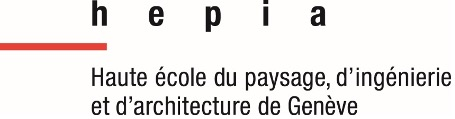
\includegraphics[height=1.29cm]{template/images/title/hepia_logo}};
	\tikz[remember picture,overlay] \node[shift={(-4.238cm,-1.97cm)}]
	at (current page.north east)
	{
\includegraphics[height=1.29cm]{template/images/title/hes-so_geneve_logo}};

\addcontentsline{toc}{chapter}{Résumé} % Adding toc entry
\thispagestyle{noheader}

\begin{spacing}{0.956}
\vspace{0.5cm}

	%% CONTENT STARTS HERE
Ce projet a pour objectif de synchroniser les arrêts de transport public présents dans OpenStreetMap avec ceux du système officiel suisse ATLAS, afin d’améliorer la précision et la fiabilité des données. Dans un premier temps, nous analysons la structure, la couverture et les balises associées des deux jeux de données, ATLAS et OpenStreetMap, spécifiquement en Suisse.

Le cœur de notre démarche repose sur un processus de correspondance sophistiqué combinant plusieurs méthodes : correspondance exacte, par nom, par distance, par itinéraire, etc. Cette approche permet d’identifier avec précision les arrêts communs aux deux bases de données. Une première analyse statistique des résultats obtenus est ensuite réalisée.

Face aux nombreux cas problématiques rencontrés, nous avons développé une application web conviviale permettant de visualiser simultanément les deux ensembles de données ainsi que leurs correspondances. Cet outil facilite l’identification des incohérences, la génération de rapports détaillés et l’exécution d’ajustements manuels pour corriger les divergences.

Le projet se conclura par la présentation des résultats finaux, définissant une stratégie claire pour atteindre une synchronisation complète entre OpenStreetMap et ATLAS. Cela garantira un ensemble de données de transport public cohérent, fiable et exploitable facilement pour divers usages.

\vfill
\begin{center}

\vfill
%% CONTENT ENDS HERE

{
%%%%%%%%%%%%%%%%%%%%%%%%%%%%%%%%%%%%%%%%%%%%%%%%%%%%%%%%%%%%%%%%%%%%%%%%%%%%%%%%
%%%%%%%%%%%%%%%%%%%%%%%%%% DO NOT MODIFY THE TABLE BELOW %%%%%%%%%%%%%%%%%%%%%%%
%%%%%%%%%%%%%%%%%%%%%%%%%%%%%%%%%%%%%%%%%%%%%%%%%%%%%%%%%%%%%%%%%%%%%%%%%%%%%%%%
	\begin{tabular*}{16cm}{p{7.59cm} p{7.58cm}}
		\small Candidat-e:					&	\small Professeur-e(s) responsable(s):\\*[10pt]
		\small\textbf{\textsc{\Author}}		&	\small\textbf{\textsc{Orestis MALASPINAS}}\\*[10pt]
		\footnotesize  Filière d’études: ISC	&	\footnotesize  \textbf{En collaboration avec:} SKI+\\*[10pt]
		\footnotesize  {} & \footnotesize  Travail de bachelor soumis à une convention de stage en entreprise: non \\*[20pt]
		\footnotesize  {} & \footnotesize  Travail soumis à un contrat de confidentialité: non\\*[10pt]
	\end{tabular*}\\*[1.9cm]
}
	
\end{center}
\end{spacing}
